\documentclass[]{article}
\usepackage{lmodern}
\usepackage{amssymb,amsmath}
\usepackage{ifxetex,ifluatex}
\usepackage{fixltx2e} % provides \textsubscript
\ifnum 0\ifxetex 1\fi\ifluatex 1\fi=0 % if pdftex
  \usepackage[T1]{fontenc}
  \usepackage[utf8]{inputenc}
\else % if luatex or xelatex
  \ifxetex
    \usepackage{mathspec}
  \else
    \usepackage{fontspec}
  \fi
  \defaultfontfeatures{Ligatures=TeX,Scale=MatchLowercase}
\fi
% use upquote if available, for straight quotes in verbatim environments
\IfFileExists{upquote.sty}{\usepackage{upquote}}{}
% use microtype if available
\IfFileExists{microtype.sty}{%
\usepackage{microtype}
\UseMicrotypeSet[protrusion]{basicmath} % disable protrusion for tt fonts
}{}
\usepackage[margin=1in]{geometry}
\usepackage{hyperref}
\hypersetup{unicode=true,
            pdftitle={Individual differences in visual perception in adults},
            pdfauthor={Rick Gilmore, Yiming Qian, \& Andrea Seisler},
            pdfborder={0 0 0},
            breaklinks=true}
\urlstyle{same}  % don't use monospace font for urls
\usepackage{longtable,booktabs}
\usepackage{graphicx,grffile}
\makeatletter
\def\maxwidth{\ifdim\Gin@nat@width>\linewidth\linewidth\else\Gin@nat@width\fi}
\def\maxheight{\ifdim\Gin@nat@height>\textheight\textheight\else\Gin@nat@height\fi}
\makeatother
% Scale images if necessary, so that they will not overflow the page
% margins by default, and it is still possible to overwrite the defaults
% using explicit options in \includegraphics[width, height, ...]{}
\setkeys{Gin}{width=\maxwidth,height=\maxheight,keepaspectratio}
\IfFileExists{parskip.sty}{%
\usepackage{parskip}
}{% else
\setlength{\parindent}{0pt}
\setlength{\parskip}{6pt plus 2pt minus 1pt}
}
\setlength{\emergencystretch}{3em}  % prevent overfull lines
\providecommand{\tightlist}{%
  \setlength{\itemsep}{0pt}\setlength{\parskip}{0pt}}
\setcounter{secnumdepth}{0}
% Redefines (sub)paragraphs to behave more like sections
\ifx\paragraph\undefined\else
\let\oldparagraph\paragraph
\renewcommand{\paragraph}[1]{\oldparagraph{#1}\mbox{}}
\fi
\ifx\subparagraph\undefined\else
\let\oldsubparagraph\subparagraph
\renewcommand{\subparagraph}[1]{\oldsubparagraph{#1}\mbox{}}
\fi

%%% Use protect on footnotes to avoid problems with footnotes in titles
\let\rmarkdownfootnote\footnote%
\def\footnote{\protect\rmarkdownfootnote}

%%% Change title format to be more compact
\usepackage{titling}

% Create subtitle command for use in maketitle
\providecommand{\subtitle}[1]{
  \posttitle{
    \begin{center}\large#1\end{center}
    }
}

\setlength{\droptitle}{-2em}

  \title{Individual differences in visual perception in adults}
    \pretitle{\vspace{\droptitle}\centering\huge}
  \posttitle{\par}
    \author{Rick Gilmore, Yiming Qian, \& Andrea Seisler}
    \preauthor{\centering\large\emph}
  \postauthor{\par}
      \predate{\centering\large\emph}
  \postdate{\par}
    \date{2019-11-07 13:19:49}


\begin{document}
\maketitle

{
\setcounter{tocdepth}{2}
\tableofcontents
}
\hypertarget{purpose}{%
\section{Purpose}\label{purpose}}

This document serves as the master protocol for the study.

\hypertarget{key-references}{%
\section{Key references}\label{key-references}}

Abramov, I., Gordon, J., Feldman, O., \& Chavarga, A. (2012). Sex \&
vision I: Spatio-temporal resolution. \emph{Biology of Sex Differences},
\emph{3}(1), 20. Retrieved from
\url{http://dx.doi.org/10.1186/2042-6410-3-20}

Murray, S. O., Schallmo, M.-P., Kolodny, T., Millin, R., Kale, A.,
Thomas, P., Rammsayer, T. H., et al. (2018). Sex differences in visual
motion processing. \emph{Current Biology}. Retrieved from
\url{http://dx.doi.org/10.1016/j.cub.2018.06.014}

\hypertarget{irb}{%
\section{IRB}\label{irb}}

This protocol, ``Individual differences in visual perception in
adults,'' has been assigned protocol number 13345. The most recent IRB
approval was granted on 2010-10-14. Files related to the approved
(exempt) submission can be found \href{../irb/2019-10-24}{here}.

\hypertarget{prior-to-data-collection-start}{%
\section{Prior to data collection
start}\label{prior-to-data-collection-start}}

\hypertarget{equipment-preparation}{%
\subsection{Equipment preparation}\label{equipment-preparation}}

First, we need to do benchmark testing to determine what screen
resolution will work at the highest temporal resolution (120 Hz). This
study requires high temporal resolution in order to measure temporal
thresholds--the shortest stimulus duration that participants require in
order to accurately detect the direction of motion.

Once we have determined the best monitor settings, we will calibrate the
monitor before we start collecting data. Those steps follow.

\hypertarget{calibrate-monitor}{%
\subsection{Calibrate Monitor}\label{calibrate-monitor}}

\hypertarget{prepare-computers}{%
\subsubsection{Prepare Computers}\label{prepare-computers}}

\begin{itemize}
\tightlist
\item
  In 503B Switch on power of large surge protector on bottom left shelf.
\end{itemize}

\hypertarget{prepare-photometer}{%
\subsubsection{Prepare Photometer}\label{prepare-photometer}}

\begin{itemize}
\tightlist
\item
  Take the photometer out of the box.
\item
  Set it up by plugging in the power and the light meter.
\item
  Turn on the photometer
\item
  Ensure the following settings:
\item
  Zero the photometer by placing the cap on the light meter and pressing
  the `zero' button
\end{itemize}

\hypertarget{start-calibrating-luminance}{%
\subsubsection{Start Calibrating
Luminance}\label{start-calibrating-luminance}}

\begin{itemize}
\item
  Turn on the computer
\item
  In 503B switch on power of large surge protector on bottom left shelf.
\item
  Log-in (Gilmore Lab)
\item
  Start Psychopy - Click icon on Task Bar
\item
  Open Monitor Settings - Go to Tools \textgreater{} Monitor Center
\item
  Click \textbf{XXXX}

  \begin{figure}
  \centering
  \includegraphics{images/new image.jpg}
  \caption{Luminance Calibration}
  \end{figure}
\item
  Enter the Monitor Screen Width in centimeters
\item
  Select \textbf{Start}\\
  \includegraphics{images/new image.jpg}
\end{itemize}

\hypertarget{calibrate-projector}{%
\subsection{Calibrate Projector}\label{calibrate-projector}}

\hypertarget{run-matlab-script}{%
\subsubsection{Run Matlab Script}\label{run-matlab-script}}

\begin{itemize}
\tightlist
\item
  At a minimum a black (0,0,0) and white (255,255,255) image must be
  displayed on the projector screen
\item
  The script to do this is located on Github:
  \url{https://gilmore-lab.github.io/photometer_proj}
\end{itemize}

\hypertarget{measure-luminance}{%
\subsubsection{Measure Luminance}\label{measure-luminance}}

\begin{itemize}
\tightlist
\item
  Measure the value of each image on the projector screen with the light
  meter.
\end{itemize}

\hypertarget{log-values}{%
\subsubsection{Log values}\label{log-values}}

\begin{itemize}
\tightlist
\item
  Log the values in the file Box
  Sync/gilmore-lab/protocols-procedures/projector-calibration.xls
\end{itemize}

We may check the monitor calibration during data collection at a
frequency we will decide later.

\hypertarget{survey-preparation}{%
\subsection{Survey preparation}\label{survey-preparation}}

This study uses Qualtrics to collect implied/oral consent and other data
from participants. Yiming has generated a draft survey, saved
\href{qualtrics_survey.qsf}{here} as a \texttt{*.qsf} format text file.

The URL for the survey is
\url{https://pennstate.qualtrics.com/jfe/form/SV_1FCXbmrfTWprQON}

\hypertarget{scheduling-participants}{%
\section{Scheduling participants}\label{scheduling-participants}}

\hypertarget{overview}{%
\subsection{Overview}\label{overview}}

Rick Gilmore is the PI on the SONA Systems study (Study ID 2587)
associated with this protocol. Yiming Qian and Andrea Seisler are
researchers. The URL is
\url{https://pennstate.sona-systems.com/exp_info.aspx?experiment_id=2587}.

The process of scheduling participants involves the following steps:

\begin{enumerate}
\def\labelenumi{\arabic{enumi}.}
\tightlist
\item
  Create slots on SONA with specific dates and times
\item
  When slot is scheduled, email sent to Yiming and Andrea.
\item
  Scheduled slots will be added to lab calendar.
\end{enumerate}

\begin{itemize}
\tightlist
\item
  The scheduled RA will be added to the title of the slot
\item
  The RA will also be invited to the google calendar event.
\end{itemize}

\begin{enumerate}
\def\labelenumi{\arabic{enumi}.}
\setcounter{enumi}{3}
\tightlist
\item
  Researchers will be contacted by email and Discord by Yiming or Andrea
  if they are needed for a slot that is not part of their regularly
  scheduled lab time.
\end{enumerate}

\hypertarget{weekly-testing-slots}{%
\subsection{Weekly testing slots}\label{weekly-testing-slots}}

\begin{longtable}[]{@{}llll@{}}
\toprule
Day of Week & Time & Researcher(s) & Lead\tabularnewline
\midrule
\endhead
Mon & 09:00a & Rachel & Andrea\tabularnewline
& 10:15a & Sandy, Emily, Rachel & Andrea\tabularnewline
& 11:30a & Sandy, Emily, Amar & Yiming\tabularnewline
& 1p & & Yiming\tabularnewline
& 2:15p & & Yiming\tabularnewline
& 3:30p & & Yiming\tabularnewline
& 4:45p & & Yiming\tabularnewline
Tue & 9a & Michelle, Rachel & Andrea\tabularnewline
& 10:15a & Michelle, Rachel & Andrea\tabularnewline
& 11:30a & Amar, Michelle & Andrea\tabularnewline
& 12:45p & Michelle, Joseph, Amar & Andrea\tabularnewline
Wed & 10a & Sandy, Rachel, Amar, Emily & Yiming\tabularnewline
& 11:15a & Sandy, Rachel, Amar, Emily & Andrea\tabularnewline
& 12:30p & Luka & Andrea\tabularnewline
& 1:45p & & Yiming\tabularnewline
& 3p & & Yiming\tabularnewline
& 4:15p & & Yiming\tabularnewline
& 5:30p & & Yiming\tabularnewline
Thu & 9a & Joseph, Michelle, Luka,Rachel & Yiming\tabularnewline
& 01:00p & & Yiming\tabularnewline
& 02:15p & & Yiming\tabularnewline
& 03:30p & & Yiming\tabularnewline
& 04:45p & & Yiming\tabularnewline
Tue & 09:00a & Michelle, Rachel & Andrea\tabularnewline
& 10:15a & Michelle, Rachel & Andrea\tabularnewline
& 11:30a & Amar, Michelle & Andrea\tabularnewline
& 12:45p & Michelle, Joseph, Amar & Andrea\tabularnewline
Wed & 10:00a & Sandy, Rachel, Amar & Yiming\tabularnewline
& 11:15a & Sandy, Rachel, Amar, Emily & Andrea\tabularnewline
& 12:30p & Luka & Andrea\tabularnewline
& 01:45p & & Yiming\tabularnewline
& 03:00p & & Yiming\tabularnewline
& 04:15p & & Yiming\tabularnewline
& 05:30p & & Yiming\tabularnewline
Thu & 09:00a & Joseph, Michelle, Luka,Rachel & Yiming\tabularnewline
& 10:15 & Rachel & Yiming\tabularnewline
& 11:30a & Amar & Yiming\tabularnewline
& 01:30p & Luka & Yiming\tabularnewline
& 02:45p & & Yiming\tabularnewline
& 04:00p & & Yiming\tabularnewline
& 05:15p & & Yiming\tabularnewline
Fri & 09:00a & Rachel & Yiming\tabularnewline
& 10:15a & Rachel, Emily, Amar & Yiming\tabularnewline
& 11:30a & Rachel, Emily, Amar & Andrea\tabularnewline
& 12:45p & Emily, Amar & Andrea\tabularnewline
& 02:00p & Michelle & Yiming\tabularnewline
& 03:15p & & Yiming\tabularnewline
& 04:30p & & Yiming\tabularnewline
\bottomrule
\end{longtable}

\hypertarget{day-of-visit}{%
\section{Day of visit}\label{day-of-visit}}

\hypertarget{before-participant-arrives}{%
\subsection{Before participant
arrives}\label{before-participant-arrives}}

\begin{itemize}
\tightlist
\item
  Check to see if there have been any cancellations.
\item
  If the scheduled study is still on the books, proceed as follows.
\end{itemize}

\hypertarget{set-up-for-vision-screening}{%
\subsubsection{Set-up for Vision
Screening}\label{set-up-for-vision-screening}}

\hypertarget{preparation}{%
\paragraph{Preparation}\label{preparation}}

Materials for vision screening are stored on the table next to Andrea's
office.

\begin{itemize}
\tightlist
\item
  Make sure the black tape is on the floor 10ft from the HOVT Snellen
  Acuity Chart which is on the door to 503B
\item
  Place Stereo Acuity Test and Glasses on table
\item
  Place Color Vision Test on table
\item
  Place the Vision Screening Score Sheet on the table
\end{itemize}

\hypertarget{review-vision-screening-procedures}{%
\paragraph{Review vision screening
procedures}\label{review-vision-screening-procedures}}

The vision screening protocol may be reviewed at
\href{vision-screening-protocol.html}{this link}

\hypertarget{set-up-for-computer-based-tasks}{%
\subsubsection{Set up for computer-based
tasks}\label{set-up-for-computer-based-tasks}}

\hypertarget{stimuli-computer}{%
\paragraph{Stimuli Computer}\label{stimuli-computer}}

\begin{itemize}
\tightlist
\item
  \emph{Log into Data Collection Computer}

  \begin{itemize}
  \tightlist
  \item
    Turn on the power of the data collection computer
  \item
    Turn on the CRT monitor in 503B
  \item
    Log-in (Gilmore Lab)
  \end{itemize}
\item
  \emph{Start Psychopy}

  \begin{itemize}
  \tightlist
  \item
    Click \textbf{PsychoPy} icon on Task Bar
    
\includegraphics{images/PsychoPy-1.PNG}\\
  \end{itemize}
\item
  \emph{Double-check monitor settings within Windows}

  \begin{itemize}
  \tightlist
  \item
    Click Settings (`gear') icon on Task Bar
    
\includegraphics{images/DispSettings-1.PNG}\\
  \item
    Choose \textbf{System}\\
    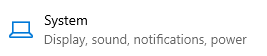
\includegraphics{images/DS2.PNG}\\
  \item
    Choose \textbf{Display}\\
    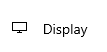
\includegraphics{images/ds3.PNG}\\
  \item
    Choose \textbf{Advanced display settings} (You may need to scroll
    down to see this)\\
    
\includegraphics{images/DS4.PNG}\\
  \item
    Make sure the window that appears has the following Settings
    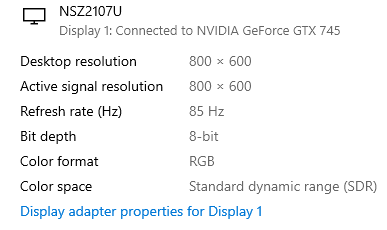
\includegraphics{images/ds5.PNG}\\
  \end{itemize}
\item
  \emph{Double-check Brightness/Contrast of monitor}

  \begin{itemize}
  \item
    Contrast:
  \item
    Brightness:
  \item
    Press any button on the monitor (except Signal A/B/OSD OFF and the
    Power button)
  \item
    Navigate to the leftmost option in the settings menu (looks like a
    half moon)
  \item
    Press the down button on the monitor
  \item
    Adjust the Contrast (leftmost option) to the required setting using
    the +/- buttons on the monitor
  \item
    Adjust the Brightness (second option from the left) to the required
    setting using the +/- buttons on the monitor
  \end{itemize}
\item
  \emph{Check monitor within PsychoPy}

  \begin{itemize}
  \tightlist
  \item
    Go to \textbf{Monitor Settings} 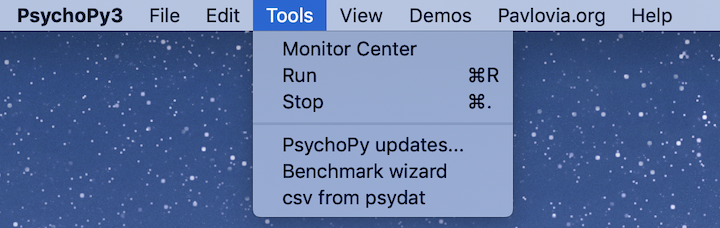
\includegraphics{images/pp2.png}
  \item
    View Settings, they should be as follows\\
    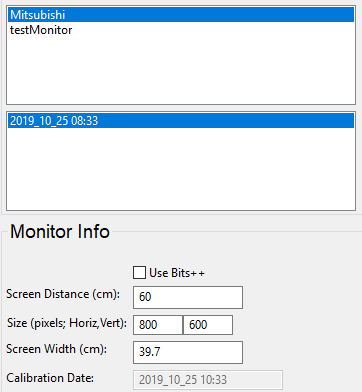
\includegraphics{images/pp3.PNG}
  \end{itemize}
\end{itemize}

\hypertarget{survey-computer}{%
\paragraph{Survey Computer}\label{survey-computer}}

\begin{itemize}
\tightlist
\item
  Log-in to survey computer
\item
  Load page with surveys:
  \url{https://pennstate.qualtrics.com/jfe/form/SV_1FCXbmrfTWprQON}
\end{itemize}

\hypertarget{after-participant-arrives}{%
\subsubsection{After participant
arrives}\label{after-participant-arrives}}

\hypertarget{welcome-participant}{%
\paragraph{Welcome participant}\label{welcome-participant}}

Say:

\begin{quote}
``\emph{Welcome to the brain, behavior, and development lab. Are you
hear for the study about motion perception?}''
\end{quote}

If the participant answers yes, say:

\begin{quote}
``\emph{Great. You can put your coat on the back of the door and your
bag here.}''
\end{quote}

\begin{itemize}
\tightlist
\item
  Store coat on back of main door and bags by the file/bookcase.
\end{itemize}

\begin{quote}
``\emph{Are you \textless{}NAME OF PERSON ON SONA SYSTEMS SITE SCHEDULED
FOR THIS SESSION\textgreater{}?}''
\end{quote}

\begin{itemize}
\tightlist
\item
  If the participant answers yes, say:
\end{itemize}

\begin{quote}
``\emph{Ok. We want to make sure that you get credit for participation.
Please sit here for the first portion of the study.}''
\end{quote}

\begin{itemize}
\tightlist
\item
  Have the person sit at the computer where the survey will be taken.
\end{itemize}

\hypertarget{begin-the-survey}{%
\paragraph{Begin the survey}\label{begin-the-survey}}

\begin{itemize}
\tightlist
\item
  Enter the ID: YYYY-MM-DD-HHMM based on appointment time
\end{itemize}

Conduct the implied verbal consent. You may say to the participant or
have them read the following text:

You are being invited to volunteer to participate in a research study.
This summary explains information about this research.

\begin{itemize}
\tightlist
\item
  The purpose of this voluntary research study is to investigate how
  human beings perceive motion in an experimental setting and how this
  ability is related to personal interests and other abilities. The
  results of this research study will help scientists gain a deeper
  understanding of what contributes to individual differences in motion
  perception, and whether or how motion perception is correlated with
  other aspects of life.
\item
  You will complete some computer-based surveys about your background,
  personal interests, spatial and verbal abilities (\textasciitilde{}25
  min). Then, you will complete one or two short (10-20 min) computer
  tasks in which you will attempt to detect motion or recognize the
  direction of motion presented on a computer screen.
\item
  All questionnaire and computer task data you provide will be saved
  using a numeric code. No information about your identity or how to
  contact you will be saved with the data.
\item
  If you are participating as part of the Psychology Subject Pool, you
  will receive course credit for participating (at the rate of ½ credit
  per ½ hours) as specified in the syllabus provided by your instructor.
  This means you will get 1 credit for participating this research.
  Alternative means for earning this course credit are available as
  specified in the syllabus.
\end{itemize}

If you have questions, complaints, or concerns about the research, you
should contact Yiming Qian at 814-863-3116 or Rick Gilmore at
814-865-3664. If you have questions regarding your rights as a research
subject or concerns regarding your privacy, you may contact the Office
for Research Protections at 814-865-1775.

Your participation is voluntary and you may decide to stop at any time.
You do not have to answer any questions that you do not want to answer.

Clicking the ``Take The Survey'' button implies two things: (1) that you
are at least 18 years of age, and (2) you voluntarily consent to
participate in the research. Thank you!

Once the consent is complete, say:

\begin{quote}
``\emph{That's great. Now we'd like to move on to the vision screening
portion of the study. Are you ready?}''
\end{quote}

\begin{itemize}
\tightlist
\item
  If the participant says yes, proceed.
\end{itemize}

\hypertarget{complete-pattern-visual-acuity-testing}{%
\subsubsection{Complete pattern visual acuity
testing}\label{complete-pattern-visual-acuity-testing}}

\begin{itemize}
\tightlist
\item
  Complete \href{vision-screening-protocol.html}{pattern acuity test}

  \begin{itemize}
  \tightlist
  \item
    Adult - HOTV @ 10ft
  \end{itemize}
\end{itemize}

\hypertarget{questionnaires}{%
\subsubsection{Questionnaires}\label{questionnaires}}

\begin{quote}
``\emph{Thank you. Now we'd like to move on to the questionnaire portion
of the study. Are you ready?}''
\end{quote}

\begin{itemize}
\tightlist
\item
  Have the participant sit back down at the computer.
\item
  Let the participants finish the questionnaire.
\item
  Ask the participant if they need a little break. If the participant
  wants to keep going, lead them to the test room
\end{itemize}

Say:

\begin{quote}
``\emph{You have finished the first part of testing. Next you have
behavorial testing. Do you want to continue or have a little break?}''
\end{quote}

\hypertarget{set-up-for-computer-based-tasks-1}{%
\subsubsection{Set-up for computer-based
tasks}\label{set-up-for-computer-based-tasks-1}}

\begin{itemize}
\tightlist
\item
  Guide participant to the testing room.
\item
  Have them sit in the chair.
\item
  Adjust the monitor and participant position.
\item
  The monitor should be located \textbf{60cm} from the bridge of the
  nose on the participant.
\item
  The chair height should be set so the participant is looking in the
  middle of the screen.
\item
  Guide the participant to use the arrow keys for responses and the
  space bar to advance the screen.
\end{itemize}

\hypertarget{run-computer-based-tasks}{%
\subsubsection{Run computer-based
tasks}\label{run-computer-based-tasks}}

\hypertarget{select-run-order}{%
\paragraph{Select run order}\label{select-run-order}}

The order of the computer experiments will be randomized across
participants in Qualtrics - run the Murray et al.~task first - run the
Abramov et al.~task first. \emph{Record the task run first on the
experiment run log.}

\hypertarget{murray-et-al.}{%
\paragraph{Murray et al.}\label{murray-et-al.}}

\begin{itemize}
\tightlist
\item
  Open PsychoPy by clicking on the icon located on the desktop.
  
\includegraphics{images/PsychoPy-1.PNG}\\
\item
  When PsychoPy opens, open the file for this experiment.

  \begin{itemize}
  \tightlist
  \item
    From the \texttt{File} menu, select the \texttt{Open\ Recent...}
    command and select the \texttt{motion-temporal-threshold.py} file.
  \end{itemize}
\item
  When the file opens, run the experiment by pressing press the green
  (running person) button. 
\includegraphics{images/PPrunningMan.png}

  \begin{itemize}
  \tightlist
  \item
    \textbf{Be careful not to type in the programming window.}
  \item
    A welcome screen with the following message will appear:
    \emph{Welcome to the motion duration threshold study. Press any key
    to continue.}
  \end{itemize}
\item
  When you are ready to enter the participant ID, press a key on the
  keyboard.

  \begin{itemize}
  \tightlist
  \item
    A pop-up window will appear.
  \item
    Enter the participant ID and gender in the pop window, and press the
    \texttt{Ok} button to enter the data.
  \end{itemize}
\item
  Speak to the participant
\end{itemize}

\begin{quote}
``In this task, you will try to detect whether a small patch of stripes
is moving to the left or to the right. The time the patch appears on the
display will get shorter and shorter. Our goal is to find out the
shortest duration you need to reliably detect the direction of motion.''
\end{quote}

\begin{quote}
``This task takes about 2 min to complete. But to make sure that we get
reliable results, we'll need to do it 4 times. You can take a short
break between the sections.''
\end{quote}

\begin{quote}
``Put your fingers on the left and right arrow keys. You'll press the
left arrow if you see motion to the left and the right arrow if you see
motion to the right. If you aren't sure, make your best guess.''
\end{quote}

\begin{quote}
``Remember, accuracy is more important that speed. Please take your
time.''
\end{quote}

\begin{quote}
``Are you ready. Ok, let's go.''
\end{quote}

\hypertarget{abramov-et-al.}{%
\paragraph{Abramov et al.}\label{abramov-et-al.}}

\begin{itemize}
\tightlist
\item
  Open PsychoPy by clicking on the icon located on the desktop.
  
\includegraphics{images/PsychoPy-1.PNG}\\
\item
  When PsychoPy opens, open the file for this experiment.

  \begin{itemize}
  \tightlist
  \item
    From the \texttt{File} menu, select the \texttt{Open\ Recent...}
    command and select the \texttt{xxx.py} file.
  \end{itemize}
\item
  When the file opens, run the experiment by pressing press the green
  (running person) button. 
\includegraphics{images/PPrunningMan.png}

  \begin{itemize}
  \tightlist
  \item
    \textbf{Be careful not to type in the programming window.}
  \item
    A welcome screen with the following message will appear:
    \emph{Welcome to the motion duration threshold study. Press any key
    to continue.}
  \end{itemize}
\item
  When you are ready to enter the participant ID, press a key on the
  keyboard.

  \begin{itemize}
  \tightlist
  \item
    A pop-up window will appear.
  \item
    Enter the participant ID and gender in the pop window, and press the
    \texttt{Ok} button to enter the data.
  \end{itemize}
\item
  Speak to the participant
\end{itemize}

\begin{quote}
``In this task, you will try to detect the direction of a small patch of
black and white strips are vertical or horizontal. The width of the
stripes will get smaller and smaller. Our goal is to find out the
smallest stripe width that you need to reliably detect the direction of
stripes.''
\end{quote}

\begin{quote}
``This task takes about 2 min to complete. But to make sure that we get
reliable results, we'll need to do it 4 times. You can take a short
break between the sections.''
\end{quote}

\begin{quote}
``Put your fingers on the down and right arrow keys. You'll press the
right arrow if you see horizontal stripes and the down arrow if you see
vertical stripes If you aren't sure, make your best guess.''
\end{quote}

\begin{quote}
"After you see the black dot, you will press the space bar to start the
trial and wait for the white dot to appear to respond.
\end{quote}

\begin{quote}
``Remember, accuracy is more important that speed. Please take your
time.''
\end{quote}

\begin{quote}
``Are you ready. Ok, let's go.''
\end{quote}

\hypertarget{optional-stereo-acuity-and-color-vision-tests}{%
\subsubsection{(Optional) stereo acuity and color vision
tests}\label{optional-stereo-acuity-and-color-vision-tests}}

If there is time left (5 min before the end of the 1 hr session),

\begin{quote}
``\emph{Thank you so much. It looks like we have time for two more short
vision tests. Please come sit over here at this table.}''
\end{quote}

Escort participant to table.

\begin{itemize}
\tightlist
\item
  Complete \href{vision-screening-protocol.html}{Stereo Acuity Test}
\item
  Complete \href{vision-screening-protocol.html}{Color Vision Test}
\end{itemize}

\hypertarget{after-session-ends}{%
\subsection{After session ends}\label{after-session-ends}}

\hypertarget{thank-participant}{%
\subsubsection{Thank participant}\label{thank-participant}}

\begin{itemize}
\tightlist
\item
  After the participant finishes all the tests, thank him/her.
\end{itemize}

\begin{quote}
``\emph{Thank you for participating this experiment. We appreciate your
time. Do you have any questions?}''
\end{quote}

\begin{itemize}
\tightlist
\item
  Answer any questions the participant might have. You may direct them
  to Yiming or to Dr.~Gilmore if you are unable to answer the question.
\end{itemize}

\hypertarget{give-participant-credit-on-sona}{%
\subsubsection{Give participant credit on
SONA}\label{give-participant-credit-on-sona}}

\begin{itemize}
\tightlist
\item
  Yiming or Andrea will assign credit in SONA.
\end{itemize}

\hypertarget{clean-up}{%
\subsubsection{Clean-up}\label{clean-up}}

\begin{itemize}
\tightlist
\item
  Clean keyboard, mouse and table and begin
  \href{sex-differences-data-export.md}{data export} (separate
  protocols).
\end{itemize}

\hypertarget{data-processing}{%
\section{Data processing}\label{data-processing}}

\hypertarget{gathering}{%
\subsection{Gathering}\label{gathering}}

\hypertarget{retrieve-behavioral-data}{%
\subsubsection{Retrieve Behavioral
Data}\label{retrieve-behavioral-data}}

\begin{itemize}
\tightlist
\item
  Output data files from the computer task are stored

  \begin{itemize}
  \tightlist
  \item
    /Documents/PsychoPy-Stimuli/\textbf{Murray Folder Name}/csv
  \item
    /Documents/PsychoPy-Stimuli/\textbf{Abramov Folder Name}/data
  \end{itemize}
\item
  Data must be copied to the \textbf{Gilmore Lab Participant Data} drive
  from the testing PC.
\item
  Data will be copied to Box (XXX).
\item
  After data export is complete, turn off computer and monitor in 503B.
\end{itemize}

\hypertarget{retrieve-qualtrics-data}{%
\subsubsection{Retrieve Qualtrics Data}\label{retrieve-qualtrics-data}}

\begin{itemize}
\tightlist
\item
  Log in to Qualtrics \url{https://pennstate.qualtrics.com/}

  \begin{itemize}
  \tightlist
  \item
    To review total summary, which shows total graph summary of survey
    distribution

    \begin{itemize}
    \tightlist
    \item
      Click on \textbf{Distributions} tab
    \end{itemize}
  \item
    To review individual responses to survey questions
  \item
    Click on \textbf{Data \& Analysis} tab
  \item
    Under \textbf{Actions} click to open drop down menu
  \item
    Click \textbf{view response}
  \end{itemize}
\end{itemize}

\hypertarget{transfer-vision-screening-data}{%
\subsubsection{Transfer vision screening
data}\label{transfer-vision-screening-data}}

\begin{itemize}
\tightlist
\item
  Vision Screening Data will be entered into the last page of the
  Qualtrics Survey.
\end{itemize}

\hypertarget{validation-and-cleaning}{%
\subsection{Validation and cleaning}\label{validation-and-cleaning}}

The \texttt{analysis/session\_qa.Rmd} script imports a data file
specified as an input parameter, for example:
\texttt{rmarkdown::render(\textquotesingle{}analysis/session\_qa.Rmd\textquotesingle{},\ params\ =\ list(data\_fn=\textquotesingle{}2019-10-29-140253\_temp\_thresh.csv\textquotesingle{}))}.
The script should be improved to output a custom HTML or PDF report for
each participant file. To view an example, visit
\href{https://gilmore-lab.github.io/sex-differences-in-motion-perception/analysis/session_qa.html}{this
link}.

\hypertarget{visualization}{%
\subsection{Visualization}\label{visualization}}

\hypertarget{analysis}{%
\subsection{Analysis}\label{analysis}}

\hypertarget{appendices}{%
\section{Appendices}\label{appendices}}

\hypertarget{purpose-1}{%
\subsection{Purpose}\label{purpose-1}}

This following explains the terminology we use in this study.

\hypertarget{terms}{%
\subsection{Terms}\label{terms}}

\hypertarget{contrast-sensitivity-function-csf-task}{%
\subsubsection{Contrast-sensitivity function (CSF)
task}\label{contrast-sensitivity-function-csf-task}}

This is the spatio-temporal constrast sensitivity function task from
\href{https://doi.org/10.1186/2042-6410-3-20}{Abramov et al}.

\hypertarget{temporal-threshold-task}{%
\subsubsection{Temporal threshold task}\label{temporal-threshold-task}}

This is the temporal threshold task from
\href{https://doi.org/10.1016/j.cub.2018.06.014}{Murray et al}.

\hypertarget{qualtrics}{%
\subsubsection{Qualtrics}\label{qualtrics}}

\hypertarget{psychopy}{%
\subsubsection{PsychoPy}\label{psychopy}}

\hypertarget{sona-systems}{%
\subsubsection{SONA Systems}\label{sona-systems}}

\hypertarget{purpose-2}{%
\subsection{Purpose}\label{purpose-2}}

The following summarizes the display and experimental parameters for the
two studies in order to clarify which ones we have chosen for our
replication.

Abramov, I., Gordon, J., Feldman, O., \& Chavarga, A. (2012). Sex \&
vision I: Spatio-temporal resolution. \emph{Biology of Sex differences},
\emph{3}(1), 20. bsd.biomedcentral.com. Retrieved from
\url{http://dx.doi.org/10.1186/2042-6410-3-20}

Murray, S. O., Schallmo, M.-P., Kolodny, T., Millin, R., Kale, A.,
Thomas, P., Rammsayer, T. H., et al. (2018). Sex differences in visual
motion processing. \emph{Current Biology}, Retrieved from
\url{http://dx.doi.org/10.1016/j.cub.2018.06.014}

\hypertarget{murray-et-al.-1}{%
\subsection{Murray et al.}\label{murray-et-al.-1}}

\begin{itemize}
\tightlist
\item
  contrast levels (low = 3\%, high = 98\%)
\item
  Diameter = 0.84, 1.7 and 10°
\item
  Motion speed was 4 cycles/s (Hz)
\item
  spatial frequency was 1.2 cycles/°.
\item
  Gratings were presented within a circular aperture, whose edges were
  blurred with a Gaussian envelope (SD = 0.21°)
\item
  Trials began with a central fixation mark, a small shrinking circle
  (850 ms).
\item
  This was followed by a blank screen (150 ms)
\item
  after which the grating stimuli appeared (variable duration controlled
  by a staircase procedure, range 6.7 -- 333 ms)
\item
  followed by another blank screen (150 ms), and finally a fixation mark
  (the response cue)
\end{itemize}

\hypertarget{abramov-et-al.2012}{%
\subsection{Abramov et al.~2012}\label{abramov-et-al.2012}}

\hypertarget{tabular-comparison}{%
\subsection{Tabular comparison}\label{tabular-comparison}}

\begin{longtable}[]{@{}lll@{}}
\toprule
\begin{minipage}[b]{0.36\columnwidth}\raggedright
Parameter\strut
\end{minipage} & \begin{minipage}[b]{0.29\columnwidth}\raggedright
Abramov\strut
\end{minipage} & \begin{minipage}[b]{0.26\columnwidth}\raggedright
Murray\strut
\end{minipage}\tabularnewline
\midrule
\endhead
\begin{minipage}[t]{0.36\columnwidth}\raggedright
Stimulus\strut
\end{minipage} & \begin{minipage}[t]{0.29\columnwidth}\raggedright
grating\strut
\end{minipage} & \begin{minipage}[t]{0.26\columnwidth}\raggedright
grating\strut
\end{minipage}\tabularnewline
\begin{minipage}[t]{0.36\columnwidth}\raggedright
Spatial frequency (cyc/\(^{\circ}\))\strut
\end{minipage} & \begin{minipage}[t]{0.29\columnwidth}\raggedright
0.6, 1, 2, 5, 12, 24.4\strut
\end{minipage} & \begin{minipage}[t]{0.26\columnwidth}\raggedright
1(UR\footnotemark{}), 1.2(UW\footnotemark{})\strut
\end{minipage}
\addtocounter{footnote}{-1}
\footnotetext{University of Washington cohort}
\addtocounter{footnote}{1}
\footnotetext{University of Rochester cohort}\tabularnewline
\begin{minipage}[t]{0.36\columnwidth}\raggedright
Temporal frequency (cyc/s; Hz)\strut
\end{minipage} & \begin{minipage}[t]{0.29\columnwidth}\raggedright
1, 4, 8, 15, 24\strut
\end{minipage} & \begin{minipage}[t]{0.26\columnwidth}\raggedright
4(UW)\strut
\end{minipage}\tabularnewline
\begin{minipage}[t]{0.36\columnwidth}\raggedright
Speed (cyc/s)\strut
\end{minipage} & \begin{minipage}[t]{0.29\columnwidth}\raggedright
\strut
\end{minipage} & \begin{minipage}[t]{0.26\columnwidth}\raggedright
4(UR), 4.8(UB\footnotemark{})\strut
\end{minipage}
\footnotetext{University of Bern cohort}\tabularnewline
\begin{minipage}[t]{0.36\columnwidth}\raggedright
Contrast\strut
\end{minipage} & \begin{minipage}[t]{0.29\columnwidth}\raggedright
via staircase\strut
\end{minipage} & \begin{minipage}[t]{0.26\columnwidth}\raggedright
0.3\%(UW), 42\%(UR), 95\%(UB), 98(UW)\%\strut
\end{minipage}\tabularnewline
\begin{minipage}[t]{0.36\columnwidth}\raggedright
Contrast modulation\strut
\end{minipage} & \begin{minipage}[t]{0.29\columnwidth}\raggedright
sinusoidal counterphase\strut
\end{minipage} & \begin{minipage}[t]{0.26\columnwidth}\raggedright
left/right motion\strut
\end{minipage}\tabularnewline
\begin{minipage}[t]{0.36\columnwidth}\raggedright
Temporal onset\strut
\end{minipage} & \begin{minipage}[t]{0.29\columnwidth}\raggedright
0.5s ramp up; 1s steady at max contrast; 0.5s ramp down\strut
\end{minipage} & \begin{minipage}[t]{0.26\columnwidth}\raggedright
trapezoidal rise, steady, decline\strut
\end{minipage}\tabularnewline
\begin{minipage}[t]{0.36\columnwidth}\raggedright
Mask/shape\strut
\end{minipage} & \begin{minipage}[t]{0.29\columnwidth}\raggedright
circular\strut
\end{minipage} & \begin{minipage}[t]{0.26\columnwidth}\raggedright
gaussian, SD=0.21\(^{\circ}\)(UW), raised cosine(UR, UB)\strut
\end{minipage}\tabularnewline
\begin{minipage}[t]{0.36\columnwidth}\raggedright
Size (\(^{\circ}\))\strut
\end{minipage} & \begin{minipage}[t]{0.29\columnwidth}\raggedright
3.5\strut
\end{minipage} & \begin{minipage}[t]{0.26\columnwidth}\raggedright
0.85(UW), 1.7(UW), 2(UR, UB), 4(UR, UB), 6(UB), 8(UR, UB), 10(UW)\strut
\end{minipage}\tabularnewline
\begin{minipage}[t]{0.36\columnwidth}\raggedright
Surround\strut
\end{minipage} & \begin{minipage}[t]{0.29\columnwidth}\raggedright
White 13\(^{\circ}\) x 13\(^{\circ}\)\strut
\end{minipage} & \begin{minipage}[t]{0.26\columnwidth}\raggedright
\strut
\end{minipage}\tabularnewline
\begin{minipage}[t]{0.36\columnwidth}\raggedright
View distance\strut
\end{minipage} & \begin{minipage}[t]{0.29\columnwidth}\raggedright
3600cm\strut
\end{minipage} & \begin{minipage}[t]{0.26\columnwidth}\raggedright
66cm(UW), 146cm(UR)\strut
\end{minipage}\tabularnewline
\begin{minipage}[t]{0.36\columnwidth}\raggedright
Task\strut
\end{minipage} & \begin{minipage}[t]{0.29\columnwidth}\raggedright
Orientation discrimination: horizontal/vertical\strut
\end{minipage} & \begin{minipage}[t]{0.26\columnwidth}\raggedright
Direction discrimination: left/right\strut
\end{minipage}\tabularnewline
\begin{minipage}[t]{0.36\columnwidth}\raggedright
Response period\strut
\end{minipage} & \begin{minipage}[t]{0.29\columnwidth}\raggedright
Unlimited\strut
\end{minipage} & \begin{minipage}[t]{0.26\columnwidth}\raggedright
\strut
\end{minipage}\tabularnewline
\begin{minipage}[t]{0.36\columnwidth}\raggedright
Feedback\strut
\end{minipage} & \begin{minipage}[t]{0.29\columnwidth}\raggedright
Auditory (correct trials)\strut
\end{minipage} & \begin{minipage}[t]{0.26\columnwidth}\raggedright
\strut
\end{minipage}\tabularnewline
\begin{minipage}[t]{0.36\columnwidth}\raggedright
Training trials\strut
\end{minipage} & \begin{minipage}[t]{0.29\columnwidth}\raggedright
No\strut
\end{minipage} & \begin{minipage}[t]{0.26\columnwidth}\raggedright
\strut
\end{minipage}\tabularnewline
\begin{minipage}[t]{0.36\columnwidth}\raggedright
Staircase algorithm\strut
\end{minipage} & \begin{minipage}[t]{0.29\columnwidth}\raggedright
QUEST\strut
\end{minipage} & \begin{minipage}[t]{0.26\columnwidth}\raggedright
Psi(UW), QUEST(UR, UB)\strut
\end{minipage}\tabularnewline
\begin{minipage}[t]{0.36\columnwidth}\raggedright
Staircase trials\strut
\end{minipage} & \begin{minipage}[t]{0.29\columnwidth}\raggedright
\strut
\end{minipage} & \begin{minipage}[t]{0.26\columnwidth}\raggedright
30 + 10 catch trials, 44(UB)\strut
\end{minipage}\tabularnewline
\begin{minipage}[t]{0.36\columnwidth}\raggedright
Threshold parameters\strut
\end{minipage} & \begin{minipage}[t]{0.29\columnwidth}\raggedright
\strut
\end{minipage} & \begin{minipage}[t]{0.26\columnwidth}\raggedright
80\%(UR), 82\%(UB)\strut
\end{minipage}\tabularnewline
\begin{minipage}[t]{0.36\columnwidth}\raggedright
\(n\) staircases/condition\strut
\end{minipage} & \begin{minipage}[t]{0.29\columnwidth}\raggedright
\strut
\end{minipage} & \begin{minipage}[t]{0.26\columnwidth}\raggedright
4(UW), 2 practice + 6(UR), 6(UB)\strut
\end{minipage}\tabularnewline
\begin{minipage}[t]{0.36\columnwidth}\raggedright
Threshold calculation\strut
\end{minipage} & \begin{minipage}[t]{0.29\columnwidth}\raggedright
\strut
\end{minipage} & \begin{minipage}[t]{0.26\columnwidth}\raggedright
median of 4(UW); drop high+low then mean of 4(UR), drop high+low then
mean of 4(UB)\strut
\end{minipage}\tabularnewline
\bottomrule
\end{longtable}

\hypertarget{replication-parameters}{%
\subsection{Replication parameters}\label{replication-parameters}}

\hypertarget{criteria}{%
\subsubsection{Criteria}\label{criteria}}

\begin{enumerate}
\def\labelenumi{\arabic{enumi}.}
\tightlist
\item
  Parameters that \textbf{maximize} sex differences.
\item
  Parameters that \textbf{minimize} sex differences.
\item
  Parameters that permit comparison between the two paradigms.
\end{enumerate}

\hypertarget{choices-and-justification}{%
\subsubsection{Choices and
justification}\label{choices-and-justification}}

\hypertarget{abramov}{%
\paragraph{Abramov}\label{abramov}}

\begin{enumerate}
\def\labelenumi{\arabic{enumi}.}
\tightlist
\item
  Maximize differences
\end{enumerate}

\begin{itemize}
\tightlist
\item
  High spatial frequency (12, 24.4 cyc/deg)
\item
  Lower temporal frequencies (1, 4, 8 Hz)
\end{itemize}

\begin{enumerate}
\def\labelenumi{\arabic{enumi}.}
\setcounter{enumi}{2}
\tightlist
\item
  Compare between paradigms
\end{enumerate}

\begin{itemize}
\tightlist
\item
  Contrast varies, so can't equate
\item
  Use 3.5 or 4 deg in diam
\item
  Use 4 Hz to equate with Murray
\item
  Can't equate spatial frequency with Murray and maximize sex difference
\item
  1 replications per condition
\end{itemize}

\hypertarget{murray}{%
\paragraph{Murray}\label{murray}}

\begin{enumerate}
\def\labelenumi{\arabic{enumi}.}
\tightlist
\item
  Maximize differences
\end{enumerate}

\begin{itemize}
\tightlist
\item
  High contrast (98\% vs.~3\%)
\item
  4 deg in diam
\end{itemize}

\begin{enumerate}
\def\labelenumi{\arabic{enumi}.}
\setcounter{enumi}{2}
\tightlist
\item
  Compare between paradigms
\end{enumerate}

\begin{itemize}
\tightlist
\item
  Used 1.2 cyc/deg, conflicts with maximizing sex differences in Abramov
\item
  3.5 or 4 deg in diam
\item
  Can't equate contrast
\item
  Use 4 Hz as in Murray
\item
  Multiple replications per condition
\end{itemize}

\hypertarget{recommendations}{%
\paragraph{Recommendations}\label{recommendations}}

\textbf{MUST} - Abramov: 12 cyc/deg, 4 Hz, 3.5 deg diam, 4 reps -
Murray: 1.2 cyc/deg, 4 Hz, 3.5 deg diam, 4 reps, 98\%contrast

\textbf{POSSIBLE, IF TIME} - Abramov: 1.2 cyc/deg (minimize sex
differences) - Murray: 3\% contrast (minimize sex difference)

\begin{itemize}
\tightlist
\item
  Decided \textbf{NOT} to have catch trials, but decide on criteria for
  dropping participants or runs based on threshold estimation.
\end{itemize}

\begin{center}\rule{0.5\linewidth}{\linethickness}\end{center}


\end{document}
